% !TXS template
\documentclass[12pt]{memoir}
\usepackage[T1]{fontenc}
\usepackage[utf8]{inputenc}
\usepackage{lmodern}
\usepackage[a4paper]{geometry}
\usepackage{graphics}
\usepackage{graphicx}
\usepackage{listings}
\usepackage{float}
\usepackage{hyperref}
\usepackage{multicol}
\setcounter{tocdepth}{3}
\setcounter{secnumdepth}{3}
\usepackage[font={small,it}]{caption}
\usepackage{subcaption}
%%\usepackage[margin=1.4in]{geometry}
%%\usepackage{babel}

%\addto\captionsfrench{% Replace "english" with the language you use
%	\renewcommand{\contentsname}%
%	{}%
%}
\renewcommand{\printtoctitle}[1]{\Huge \textbf{Table of Content}}

\renewcommand\thefigure{\arabic{figure}}
\renewcommand\thetable{\arabic{table}}
\setcounter{figure}{0}
\renewcommand{\thesection}{\arabic{section}}
\begin{document}

\title{Apprenticeship thesis, 2nd years \\ \textbf{Master of Computer Science}, speciality \textbf{Ingénierie du
		Logiciel et des Connaissances} 
	
	\bigskip
	{\huge Realtime continous optimisation of healthcare transportation fleets using massively parallele memetic algorithm on GPGPU} \\	
	}
\author{Joseph Pallamidessi\\ University of Strasbourg} 
\date{\vspace{2.5in}
	
\protect\raggedright
{\normalsize Maître d'alternance:} \\
		\textbf{Pierre Collet}, Université de Strasbourg \\
		\textbf{Guillaume Philips}, Synovo SAS}

\maketitle
\newpage

\tableofcontents*
\newpage


\section{Acknowlegments}\label{Acknowledgements}

I would first like to thank professor Collet, for the guidance provided during those
two year of apprenticeship. It is because of him that today I stand before you,
having opened to me the wonderful world of universitary research. \\
Guillaume Philip, my apprenticeship tutor inside Synovo to having me let experiment, test
and gave full liberty to conduit my research on this problem during the one and a
half year that I spent inside his company. He was always listening, throughful and
focus even when the obstacle seemed inreachable. He was flexibility, availability
and focus are something that I wish to encounter again in my carrier, as it gave me
the strength to finish this big challenge. \\
Jeremy Wies for my current position of research assistant at Synovo.
Thibault Thomas for his always optimistic mood and the overall help, on to many things to enumerate here. It was always a pleasure to discuss with him and I formally apologize for having him be me rubber ducks while being stuck on problems. As a true believer of the concept serendipity, many aspect of the current work may have been indirectly influenced by ours discussion. \\
Anne Juventy for having be a great help at a time the future of the project seemed
dire. It is be her ingenuosity and pratical minds that we were able to canalised our
thought.\\
Benjamin Chetioui for having be an efficient and resourceful coworker and his numerous inputs in all aspects of this project.


\bigskip
I would like to thanks the pedagogic team of the ILC Master and more specifically M. Narboux, M. Magaud, Mme. Mark-Zwecker for allowing me to have this unorthodox journey through theirs formation, even if it had add a lot of supplementary work on them. \\
I would like to thanks Synovo and the ICube laboratories for their support and
letting me work in this big collaboration between university researchers and the
corporate world.
Thanks to all my proofreaders and friends for taking the time to help me and theirs overall support during those last two year. \\
Finally, I wish to thanks the french university and scholastic system for making me able to pursue my eduction.  
\newpage

\section{Abstract}
We developed a distributed multi-objectives genetic algorithm for solving a special case of
large vehicle routing for healthcare service. The goal of this algorithm is to
replace the task of planification for the next day currently done by human operator and with
minor modification,due to the evolutionary nature of the used techniques, be able to
done realtime continuous optimization. The problem in itself is highly constrained
but the search space remais large enough to require heuristics. The help the
exploitation phase, a set of local searches, the most used in combinatory
optimization have been reimplemented to take into account the specificities and
multi-objective nature of the problem. \\
The optimization must be fast enough with large instance to compete with humans as
this field is  caracterised by high frequence of modification through the day . In
order to avoid the traditional computational pitfall of pareto-based selection, a
novel selection method (G-ASREA) on GPGPU has been succesfully implemented and tested with
speed-up ranging for 4 to 50 times faster than the NSGAII algorithm while providing
better population diversity and overall results.
\paragraph{Keywords}
Evolutionary algorithm, genetic algorithm, local search, GPGPU, NSGA, ASREA, multi-objective optimization, pareto selection, vehicle routing problem with time windows, Pickup-delivery, heterogeneous fleet.
\newpage
\section{Introduction}
Planification of large instance remains an open field of research. The particular
problem of vehicle routing of healthcare service is twofolds : due to its
various constraints it is difficult to extract to ontology needed for modelizing for
a linear solver and the sheer number of element to optimize make it out of reach for
the classical exact algorithm, thus the need of powerful heuristics and 
metaheuristic. The fields af vehicle routing problem (VRP) is composed of numerous variants, each time defining new constraints. The two most commons one are the Capacited Vehicle Routing Problem (CVRP) and the Vehicle routing problem with time windows (VRPTW).

\paragraph{CVRP} % (fold)
\label{par:CVRP}
In the CVRP variant, the vehicle capacity of "goods" is limited and sometime the
good must also be package in the correct of delivery, meaning it involve a knapsack
optimisation once the routing is defined.\\
This problem represent the core of logistics and is prevalent in physical goods transportation. This is also the case
of our problem as theirs is a limited number of seat in the vehicles and some
limitation concerning the ambulances for example, where theirs can be only one
patient at once, independantly of the size of the medical crew.
% paragraph CVRP (end)
%Definition of CVRP

\paragraph{VRPTW} % (fold)
\label{par:VRPTW}
In the case of delivery to consumer directly arise the question of the delivery
timing. The VRPTW is a highly constrained problem where the delivery must occurs
at specific time window. Depending of the criticality of the delivery, systems tend
to treat windows with more or less flexibility. \\ 
In our case, the delay penalty on an appointement is weighted its type. The problem definition will be given in much more
detail in the following section.
% paragraph VRPTW (end)
%Definition of VRPTW

\paragraph{Heterogenous fleet} % (fold)
\label{par:Heterogenous fleet}
Problem with heterogenous fleet add a new set of constraints. The cost of using
the vehicle, its capacity, its crew (the size as well as the diploma and
authorization required) can depend of the type of vehicle.
% paragraph Heterogenous fleet (end)
%Variant one : heterogeouns fleet

\paragraph{Multi-depot} % (fold)
\label{par:Multi-depot}
The classical definition of the VRP problem state that theirs are only one depot or
main station, from which all the vehicle start and must go back after the last
missions. In the multi-depot variant, the vehicle are assigned to a specific base,
where they start and end.\\
% paragraph Multi-depot (end)
%Variant two : Multi-depot

The more constrained the problem is the smaller the search space will be. This fact
is easy to demonstrate when graphically solving a linear integer problem with the
simplex method for example.\\
In our problem

%Genetic algorithm 
Distributed 

\section{Context of research}
\subsection{Synovo} % (fold)

Synovo est une startup strasbourgeoise crée par Jérémy Wies, fondateur,
directeur financier et commercial, Michel Lacombe, directeur Formation
\& Business Intelligence et Guillaume Phillip, directeur technique. Les
locaux de l'entreprise se situent à la Meinau, à quelque pas du lycée
Couffignal. \\ 
Jérémy Wies est le directeur et fondateur de Synovo SAS. Ancien étudiant
de Supinfo, il d'abord créé la société New Web\footnote{\url{www.new-web.fr}}, spécialiser dans les
solutions d'hébergement d'infrastructure de type cloud pour les
transporteurs sanitaire qui s'est ensuite développé avec des offres plus
généralistes puis Synovo, connaissant bien les besoins des services de
transports sanitaires. \\
L'entreprise est spécialisée dans la gestion et l'optimisation de
transport de santé en France depuis bientôt 6 ans. Leur cheval de
bataille est la gestion logistique de flotte d'ambulance destinée aux
sociétés de transport sanitaire françaises.

\bigskip
Synovo est née de l'initiative de ses trois fondateurs, alors étudiants
à SUPINFO, après avoir décroché le premier prix à un startup week-end
organisé par Strasbourg Startup en 2011. Après avoir enchainé les
concours (Yago, Talent des cités, Pépites) et levé des fonds, la société
compte maintenant plus d'une vingtaine d'employés et une dizaine de
clients répartis sur toute la France, soit un total d'environ 300
véhicules. \\
Après 3 ans de développement, leur logiciel phare, Saphir, offre une
solution de gestion aux problèmes de logistique rencontrée par ces
sociétés : prise de rendez-vous, communication entre les régulateurs et
le personnel roulant, tracking GPS, comptabilité et facturation, outils
statiques et BI. C'est dans le cadre du projet Saphir que s'intègre mon
travail de R\&D d'optimisation de tournée par algorithme génétique. La
remontée en temps réel d'information de \emph{tracker} GPS embarqués et
de l'état des missions forment un élément essentiel pour le caractère
dynamique de l'algorithme d'optimisation de tournées. \\
Mon maître
d'apprentissage et encadrant chez SYNOVO SAS est M. Guillaume Philips.
Il occupe le rôle de directeur général et de CTO. C'est avec lui que
j'ai la plupart des discussions d'ordre techniques et l'avancement du
projet HIRONDELLE. Il supervise le développement du projet Saphir dans
son ensemble.

\bigskip
L'entreprise est en pleine expansion, avec plus de 10 nouveaux employés
depuis le début de l'année portant le nombre à 23, et une vingtaine
d'embauches prévues pour la fin d'année. De nombreux étudiants d'écoles
d'informatique environnantes (Supinfo, Epitec, Exia,) viennent faire des
stages, élevant encore ce nombre. Synovo est très fortement investi dans
le tissu associatif des startups en Alsace avec des partenariats et
soutiens avec Alsace Digitale et French Tech Alsace.

\paragraph{Développement}\label{duxe9veloppement}

L'entreprise est organisée en différents pôles: support, développement,
Business intelligence, mobile et R\&D.

Le pôle développement comprend la plus grande partie de la force de
travail, soit 12 développeurs avec M. Guillaume Philips comme chef de
projet. Ce pôle se concentre sur l'ajout de nouvelles fonctionnalités au
logiciel, généralement plusieurs en parallèle.

\paragraph{Support}\label{support}

Le processus de commercialisation ayant déjà commencé et les produits
étant encore jeunes, le pôle support lui aussi composé de développeurs
C\# est de taille assez conséquente, 7 personnes environ. Leur travail
consiste à corriger les bugs remontés par les clients, à indiquer
comment utiliser certaines fonctionnalités du logiciel et à le mettre à
jour.

\paragraph{BI et ergonomie}\label{bi-et-ergonomie}

La partie d'analyses statistiques et de Business Intelligence est
dirigée par M. Michel Lacombe. Cette petite équipe (3 employées)
s'occupe aussi de tous les interfaces homme-machine de Saphir et des
produits et services connexes.

\paragraph{Mobile Android}\label{mobile-android}

2 Développeurs travaillent sur l'application mobile permettant aux
ambulanciers sur le terrain de recevoir et d'envoyer des informations
vers l'outil de régulation proposé par Saphir.

\paragraph{R\&D}\label{rd}

Cela ne fait que depuis mon arrivée en avril que Synovo dispose d'un
pôle R\&D dans ses murs. Avant cela, la partie de recherche était
fournie par l'équipe BFO du laboratoire ICube. Deux autres développeurs
m'ont rejoint en août: M. Ivan Aksamentov dans le cadre d'un stage
jusqu'à fin août et M. Benjamin Chetioui, en stage pour l'instant, qui
continuera en tant qu'apprenti dans le cadre du master d'informatique,
mention ILC.


\label{sub:Synovo}

% subsection Synovo (end)
\label{sec:Context of research}
The main motivation of this research is the automate the whole logistic process of
transporting patient for a number of reason. Historically healthcare transportation
services could not use any automation due to the large number of physicals and legal
constraints, in particular in France where the state subside part of the cost
depending on various complex conditions. This has render impossible the usage of
more traditional and top of the shelf solution available for the goods
transportation industry. Synovo, through its main product Saphir, an ERP-like tool
to manage the whole transporation company, try to push the full automation of the
industry. \\
The last remaining parts still extensibly done by humans operators are planning the
next day and doing realtime routing and problem solving during the day, two type of
work that our novel algorithm tackles efficently. The main goals to achieves are the
following:
\paragraph{Economic} % (fold)
\label{par:Economic}
A good planification that aggresively try to reduce the number of resources used
(vehicles, drivers, crews) can lead to massive saving for the transporation company
as well as improving the working condition of the current employee and preserving
the actual material.
% paragraph Economic (end)
\paragraph{Speed} % (fold)
\label{par:Speed}
For a small company, the average workload is about 100 to 200 missions (or journeys)
per day. For planning such day, it take around one hour very focused for a human
operator or regulator, while he is still interrupted by calls concerning the current
day. Before having a working planification for the next day, the company can not yet
tell its drivers and employees the beginning of theirs shifts. Having fast answer,
in the range of 5 minutes or less will be beneficial for the whole company.
% paragraph Speed (end)
\paragraph{Efficicy} % (fold)
\label{par:Efficicy}
Due to the high cognive demand of such work, the efficiency of the planning depend
in great part from the wellness of the regulator. While they are able to maintains
high quality planification during the work, the type of jobs is very exhausting on
the person. Algorithmic solutions will always have be constant in quality, and will
free the regulator to do its actual job of taking care of humans problem and
unforseeable incident on the field.

% paragraph Efficicy (end)

\subsection{Problem definition}
The problem can be caracterised as a Multi-depot Capacited Heterogeouns Pickup
Delivery Vehicle routing problem with time windows (MCHPDVRPTW). \\
Formally it can be describe this way: given a set of appointements, find the routing that minimize the
delay and lateness to serve mission, minimize the number of used vehicle, minimize
the number of used employee, while avoiding using the wrong type of vehicle,
violating legal constraint on the crews (pauses, total working time) and the number
of maximal patient in the vehicle.\\
Here is the mathematical formulation of the problem:
% Math relou ici 
%
%
\\
\\
The end goal is to be able to provided efficient optimization of the whole day in
sub 5 minutes time. That is given a set of missions, a fleet of available vehicle
and employee to get a feasable and at least human comparable planification if not
better. \\
The difficulty of such optimisation is the fact the in must optimised the vehicles
route and the employee(crews). We wanted here to take a global approach as the two
goes together and influence each other in a antagonistic way in some case, depending
of the dataset. In more ancient real-world example, the routes are optimized alone
or with very few heuristics, and a second optimisation was done on top of the result
of the first one. Such techniques even if feasable and easy to implement or test
break the promise of globally optimising the problem.\\
That is  why a multi-objective was chosen. Compared to the first working prototype
of august 2015, we changed the objective to the three following one:

\paragraph{Employee} % (fold)
\label{par:Employee}
The goal of this fitness is the reduce "cost" of the employee:

% paragraph Employee (end)

\paragraph{Vehicle} % (fold)
\label{par:Vehicle}
This objectives is designed around getting correct and working routes from the
logistic point-of-view. This mean:
\begin{itemize}
  \item Minimizing the delay of picking up and delivering patient
  \item Using the correct type of vehicle for the mission
\end{itemize}
% paragraph Vehicle (end)

\paragraph{Load} % (fold)
This fitness is kept simple in opposition to the two firsts which are agglomeration
of differents smaller fitnesses working positively correlated together. It only
evaluate the capacity of the vehicle or more exactly the overloads.
\label{par:Load}

% paragraph Load (end)

\subsubsection{Healthcare transportation specificities}
\label{sub:Healthcare transportation specificities}
In the field, healthcare transportation services take great care of having the best
quality of service. It is an industry focus on the patient comfort first, due to the
fact that patient that need transportation tends to be recurrent due to lifelong
disability or disease, such as dyalised patient which will require transportation 3
time a week during the rest of theirs life. \\
The second most important point is the feasability of the routing. Healthcare
transportation services are routinely facing the lack of resource to do all mission
and while running with low resource margin (fleet size or employee), they are
vulnerable to imprevisible incident (accident on the road, employees not showing
up).\\

As already stated earlier, the fleet of a healthcare transportation service is by
nature heterogenous. Some patient can only moved laying, while other can be sitting,
the required equipment can differ significantly: ranging from nothing to big specialized
hardware for heavy burned or morbidly obeses patient.\\
They are four type of vehicle defined by the french gouvernment, hospital and healthcare professional:

\paragraph{Vsl} % (fold)
\label{par:VSL}
A vsl (vehicle sanitaire léger or light sanitary vehicle) is a simple car, with no
other equipment than a standars medical kit. It driver must just have a driver
licence and a small certification. It is the most common type of transport, for
patient with low to no physical affliction.

\paragraph{Ambulance} % (fold)
\label{par:Ambulance}
Ambulance of heavy duty vehicle required when the patient need to be laying and need
medical attention during the travel. Ambulance are manned by a crew of two persons,
one driver and one practionner holding a DEA licence.

  \paragraph{TPMR} % (fold)
\label{par:TPMR}
A TPMR is also a king of light vehicle but setup for laying transportation. Their is
also one simple driver which didn't require any other licence. 

  \paragraph{Taxi} % (fold)
\label{par:Taxi}
A taxi is analoguous with VSL, to the point that some company don't do any
distinction between the two. The only difference is about the cost of the mission
due to heavy government subvention when satisfiying certain condition like the total
distance travel for one mission. The driver do not require any medical licences.\\
\\
The problem of patient transportation is modeled as pickup delivery vehicle routing
problem. In pickup-delivery problem, the vehicle must transport "loads" (here
patient), without any intermediatary pause, stop, change of vehicle or unloads
between the pickup phase (the origin point) and the delivery (destination).

\section{State of the project}
In september 2015, we did have a working prototype as advertised in the preceding
thesis. The core ideas and techniques have not changed between last year algorithm
and the current one, but the definition of problem did changed considerably. \\
At first, we tried to map an ontology that was very precise and did integrate a lot
the domain problematics without any treatment. This lead to sub-optimal solution,
because we were more trying to map the ontology of the problem than to solve the
problem per se. The generally confusing around the actual cost of a kilometer for
one type of vehicle, for example, and the difficulty to get estimate from transportation services
themselves proved the inefficiency of the way.\\
Because of the genericity of genetic algorithm and meta-heuristic framework, we only
had to update the domain-specific part of the algorithm: the evaluation procedure.\\
\\
Before going any further in the details, we will do a 1) quick recap of the framework
of genetic algorithm and 2) reintroduces the used operator, before jumping to the
novel part of the algorithm.

\subsection{Quick introduction to genetic algorithm} % (fold)
\label{sub:Quick introduction to genetic algorithm}
Les algorithmes génétiques (GA) sont généralement utilisés pour chercher
la meilleure solution possible à des problèmes inverse complexe,
combinatoire ou continue. \\
Ils améliorent de manière évolutive un ensemble de solutions
potentielles dans l'espace de recherche de toutes les solutions
possible. Les algorithmes génétiques ou algorithmes évolutionnaires sont
une classe d'algorithme s'inspirant de la théorie de l'évolution comme
énoncé par Charles Darwin avec son principe de \emph{« \textbf{survival
of the fittest} »}. \\ 
L'idée derrière l'utilisation et la mise en place
d'algorithmes évolutionnaires est apparue à la fin des années 50\cite{john1992adaptation} en
essayant de mimer le modèle évolutionnaire naturelle. Il a ensuite été
nécessaire d'attendre l'apparition d'ordinateur et d'unité de calcul
suffisamment puissant pour que les GA deviennent réellement
exploitables. Les analogies avec la biologie sont nombreuses. \\
Leur fonctionnement est conceptuellement très simple : la solution du
problème à résoudre est modélisée sous forme d'un individu. Une
population d'individus générés aléatoirement va être créée et cette
population va ensuite suivre la boucle évolutionnaire suivante composée
de quatre opérateurs génétiques : croisement, mutation, évaluation et
sélection. Nous les expliciterons dans quelques instants.


\subsubsection{Operator} % (fold)
\label{sub:}
\paragraph{Initialisation} % (fold)
\label{par:Initialisation}
Au début de l’algorithme, la population initiale est définie en créant des individus
aléatoires. Les GA nécessitent des générateurs de nombre aléatoire uniforme rapide et
de bonne qualité pour garantir un bon échantillonnage de l’espace de recherche comme14
les générateurs Mersenne twister ou plus récemment les xorshift[20].
Selon le problème, il peut se révéler intéressant d’introduire des contraintes ou même
des individus étant eux même des solutions de bonne qualité pour aider la recherche.
Ces biais ont néanmoins tendance à trop contraindre les solutions possibles et à perdre
la possibilité d’obtenir des résultats créatifs.
\paragraph{Crossover} % (fold)
\label{par:Crossover}
La phase de crossing-over (ou recombinaison, reproduction) consiste à créer de nou-
veaux individus d’après plusieurs parents. De nombreux types de cross-overs existent,
adaptés à diverse représentation d’individu. Le cross-over doit prendre en compte la
structure de l’individu et est de fait lui aussi spécifique au problème.

Pour corriger les problèmes du cross-over mono-point, un
\emph{cross-over} dit \textit{BCRC\cite{ombuki2006multi}} (\emph{Best cost route cross-over}) plus
récent et plus adapté au problème de \textit{ VRP} fut sélectionné pour le
remplacer de mon initiative. N'ayant pas d'implémentation disponible, il
fut d'abord prototypé en \textit{Python} à l'aide du framework évolutionnaire
\emph{DEAP} sur un problème de \emph{VRP} synthétique en utilisant les
jeu de données de VRP standard de Solomon\cite{solomon1987algorithms}. Après validation des
résultats, je l'ai porté en \textit{C++}, non sans difficulté du fait de
son utilisation massive de structure de données dynamique, délicatesse
non permise pour l'architecture \textit{GPU} visée pour des raisons de
performances. \\
Cette implémentation \emph{C++} fut la source de bien des
déboires tant au niveau de l'implémentation que des performances sur
\textit{GPU} du fait de ses nombreuses divergences et de la nécessité
d'allocation mémoire dynamique.

\begin{figure}[htbp]
	\begin{center}
		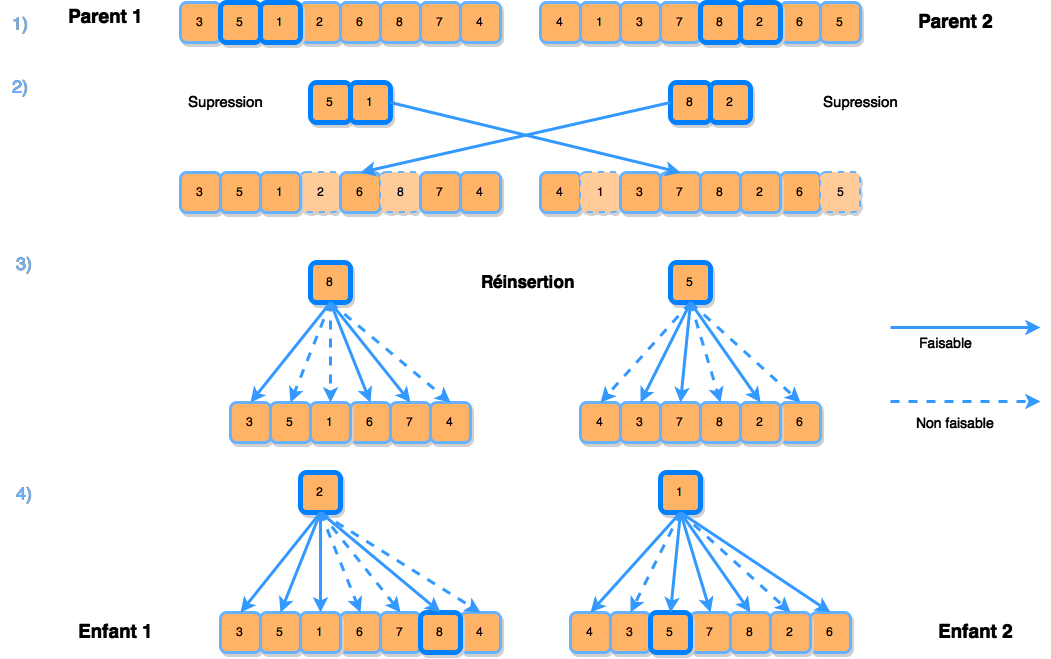
\includegraphics[width=6in]{img/BCRC.png}
		\caption{Best Cost Route Cross-over.}
	\end{center}
\end{figure}


\paragraph{Mutation} % (fold)
\label{par:Mutation}
L’opérateur de mutation permet de faire varier de manière aléatoire les nouveaux
individus « enfants » pour améliorer l’exploration de l’espace de recherche, certaines «
zones » ne sont potentiellement pas accessibles par cross-over ou lorsqu’il n’y a pas eu
d’occurrence d’un gène ou d’une certaine valeur d’un gène dans la population initiale.
Là encore, l’opérateur de mutation dépend du problème et de la représentation utilisée,
\paragraph{Evaluation} % (fold)
\label{par:Evaluation}
\paragraph{Multi-objective selection } % (fold)
Avant d'entamer la prochaine génération, il faut assigner les « nouveaux
» parents d'après l'ensemble ($\lambda$ + $\mu$) des individus enfants
$\lambda$ et des parents $\mu$ de la génération précédente. Le nombre
d'individus sélectionnés de cette manière est égal à la taille
originelle de la population parent $\mu$. \\
La sélection se base sur la \emph{fitness} des individus. Cependant, un
mécanisme simpliste où seuls les meilleurs (les plus aptes) individus
sont sélectionnés, après un tri par exemple, entraîne des problèmes de
convergence prématurée.

\bigskip
Lors du processus de sélection, il est nécessaire de garder des
individus ``relativement\cite{sharma2010archived,deb2002fast}'' bons qui aident à maintenir une certaine
diversité dans la population globale, ce qu'un choix déterministe ne
garantit pas. \\
Les méthodes de sélection sont donc généralement stochastiques comme la
très courante et efficace sélection par tournoi, qui retourne le
meilleur individu d'un ensemble aléatoire de n éléments. 
Il est à noter que les méthodes de sélection, ou sélecteurs diffèrent
grandement entre une \emph{GA} simple et une optimisation multicritère
(\emph{MOEA\footnote{Multi Objective Evolutionary Algorithm}}). Ce point précis sera bordé dans la section suivante.

\paragraph{Optimisation
multiobjectif}\label{optimisation-multiobjectif}

L'intérêt d'utiliser des algorithmes génétiques vient que les résultats
obtenus sont créatifs et compétitifs avec l'intelligence humaine. Au
bout d'un certain nombre de générations, et ce malgré le fait d'avoir
initialisé les individus aléatoirement, on obtient de « bons »
résultats. On les définit comme « bon » du fait qu'on ne peut pas
déterminer si l'optimum global du problème a été atteint ou si
l'optimisation est restée bloquée dans un optimum local. Classiquement,
on cherche à optimiser un seul critère, mais il est aussi possible d'en
avoir plusieurs possiblement antagonistes. La difficulté des algorithmes génétiques multiobjectifs (\emph{MOEA}) vient de l'opérateur de
sélection. 
\\ Dans le cas d'un algorithme mono-objectif, la sélection se
fait de manière relativement évidente : on prend les meilleurs individus
issus de multiples tournois. Avec un MOEA, comment définir un « bon »
individu ? Un individu optimisant parfaitement le critère 1 et pas les
autres est-il meilleur qu'un autre qui optimise moyennement tous les
critères ? Le principe derrière tous les opérateurs de sélection
multiobjectif (\emph{NSGA-II\cite{deb2002fast}, ASREA\cite{sharma2010archived,sharma2010gpgpu}, SPEA}) nous vient du monde de
l'économie. Il s'agit de l'optimalité de \emph{Pareto}, aussi appelée
\emph{Pareto-dominance}.

\paragraph{Dominance de Pareto}\label{dominance-de-pareto}

Dominer au sens de Pareto\cite{voorneveld2003characterization}, pour un élément donné, signifie qu'aucun
autre élément n'a au moins un critère meilleur que les siens. Dans le
cadre des \emph{MOEA}, une solution domine une autre si les deux
conditions suivantes sont remplies:

\begin{itemize}
\item
  La solution x1 n'a aucune fitness plus mauvaises que celle de x2
\item
  La solution x1 a au moins une fitness meilleure que celle de x2
\end{itemize}

\begin{figure}[htbp]
	\begin{center}
		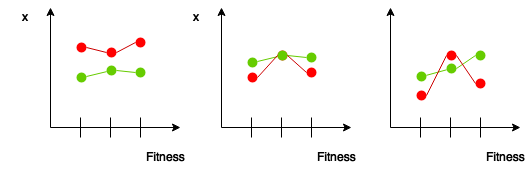
\includegraphics[width=4in]{img/paretoDominance.png}
		\caption{Soit deux individu, rouge et vert. Pour un problème de minimisation, de gauche à droite, vert domine rouge, rouge domine vert et ni rouge ni vert ne se dominent.}
	\end{center}
\end{figure}


% Plus formellement: // formule en laTex

De par cette définition on peut déduire le concept de \emph{front de
Pareto}: l'ensemble des solutions non dominé. Les fronts de Pareto
permettent de trouver de bons compromis entre les différents objectifs.
Définir un front de Pareto revient à trouver une enveloppe convexe\cite{godfrey2007algorithms} dans
un espace à dimension \textit{n}, où \textit{n} est le nombre d'objectif.

\label{par:Multi-objective selection }

\subsubsection{Parameters} % (fold)
\label{ssub:Parameter}

% subsubsection Parameter (end)
% paragraph Multi-objective selection  (end)
% paragraph Evaluation (end)
% paragraph Mutation (end)
% paragraph Crossover (end)
% paragraph Initialisation (end)
% subsection  (end)
% subsection Quick introduction to genetic algorithm (end)
Problem already finally defined 
Work already done
Small change => mainly refactoring
Genetic algorithm working fine 
In production

\section{Local searches}
By design genetic algorithm provided good exploration of the search space, meaning that they sample the fitness landspace in a coarse-grain fashion.
The mutation operator setup in the evolutionary loop, provide the smaller step of the sampling also called "exploitation". The main difficulty when trying to 
solve a problem using stochastic methods or using machine learning is to have a good ratio between exploitation and exploration. This is often refered in the literature as the sploitation/exploration problem. If the exploitation is too high, the search will be quickly stuck in local optimum and if the exploration is too high the search will not converge to any useful result. \\
With the exception of the mutation operators describe before, the first part of this thesis was focus in the exploration part of the algorithm, implemented last year. In this section we will describe the work done on creating and adapting popular local search methods in VRP and travelling saleman problem to ours specific problem as combinatory optimization often require to be help with a set of local search algorithm, small heuristics and brute force methods.

\subsection{2-opt* for pickup-delivery}
The 2-opt* local search consist of exchanging two nodes form 2 different routes. If the newly defined routes 
produced a better global solution as defined by the evaluation function (in the basic formulation of TSP 
the new solution produced a shorter global solution in distance).



\subsubsection{Base algorithm}
To avoid unneccesery computation the algorithm use the concept of tringular irregularity 
between the old and new egdes after reorganization. By doing this, there is no need to 
evaluate the whole solution after each swapping, only the locally changed resulting edge.\\
\\
The whole algorithm work as following:\\
For each node of a route, we try to swap with all the nodes of all other route and we 
select the best one as define by the evaluation function. If an improvoment over te global
 fitness occured (a swap was selected) the set a improvement boolean at true.\\
\\
We continue doing the same procedure between all the nodes of the problem, resulting in a
 complexity of O(n2). This local search, will exhaustive is greedy by nature and is not proved
 to find the best global reorganisation of nodes, which is the task of the evolutionary loop.\\
\\
Here the formulation of the algorithm.
\begin{figure}[htbp]
	\begin{center}
		\includegraphics[width=4in]{img/2-opt.png}
		\caption{Best Cost Route Cross-over.}
	\end{center}
\end{figure}
\subsubsection{2-opt*}
The 2-opt algorithm is not adapted to time-windows variant of the TSP/VRP problem like ours.
 In order to work well with the time constraint a variant of the 2-opt algorithm was developped,
 called 2-opt*. A new condition must be satisfied when swapping edge. The nodes preceding and 
following the selection one, must verify the partial order of the time-windows, greatly reducing
 the number of possible swap.\\
\\
The reformulation of the algorithm is the following:
\begin{figure}[htbp]
	\begin{center}
		\includegraphics[width=4in]{img/2-opt-star.png}
		\caption{Best Cost Route Cross-over.}
	\end{center}
\end{figure}
\subsubsection{PD-flavored version}
Unfortunalty there was not a variant for the pickup-delivery variant of the TSP/VRP problem.\\
 We decided to extends the 2-opt* local search for PD by following the same framework used to
 pass trom the 2-opt to 2-opt*. In this case the new condition to satisfied before swaping is
 he following: we swap the pickup and the delivery node of a journey simultaneously against the
 pickup or the delivery of the selected node, while satisfying the requirements of the 2-opt* 
algorithm for the two swapped node. This further reduced the possible number of swap but only 
produced legal solution.\\
\\
The reformulation of the algorithm is the following:
\\
\begin{figure}[htbp]
	\begin{center}
		\includegraphics[width=4in]{img/2-opt-star-pd.png}
		\caption{Best Cost Route Cross-over.}
	\end{center}
\end{figure}

\subsection{Intra route}
The basis of this heuristic picks two routes randomly and swaps two nodes from each route. 
Without modification this really simple heuristic will not often produce legal solution in 
the project context. We extended it by all swapping the other node of the journey with each other.\\
This is more a mutation then an heuristic as no score or recomputed in anyway. The time-windows conditions
doesn't need to by satisfied because the whole individual will be sorted following the partial order operator
for time-windows before the evalutation phase.\\
\begin{figure}[htbp]
	\begin{center}
		\includegraphics[width=6in]{img/intra.png}
		\caption{Best Cost Route Cross-over.}
	\end{center}
\end{figure}

\subsection{RAR}
An other mutation-like operator implemented the the Remove and Reinsert one. It consist of selecting randomly one node 
in a route and inserting it back to another one.Like the others, a small adaptation was necessary.
 We also remove and reinstert the sister element of the selected node. This operator is a means 
to increase the solution diversity efficiently. Contrary the actual algorithm, no feasability checks are
 done because they will occured during the evoluationary loop, in particular the crossover and 
the evaluation phase, coming right after all local searches. \\

\begin{figure}[htbp]
	\begin{center}
		\includegraphics[width=6in]{img/rar.png}
		\caption{Best Cost Route Cross-over.}
	\end{center}
\end{figure}

\subsection{Spliting and merging}
Route splitting and merging follow the same logic of the Remove and Reinsert operator.\\ 
Instead of a single node it does operate on whole section of the route. A whole section
 is remove from the original route to be reinserted to another one. Splitting and Merging are 
dual operation in the mathematical sense of the terme.\\
The difference are the following:
\begin{itemize}
  \item When splitting, the section is reinserted to an empty vehicles.
  \item When merging the section is integrated to a non-empty vehicles.
  \item Merging try to preserve the order of the subsection but abide the the time-windows partial order.
\end{itemize}
This mutation was developped because of the need to reinstate empty vehicle when optimising without
 resource minimization in mind and thus is not uselful when minimizing it. 

\begin{figure}[htbp]
\centering
	\begin{subfigure}{.5\textwidth}
                        \centering
			\includegraphics[width=2.7in]{img/merge.png}
			\caption{Best Cost Route Cross-over.}
	
	\end{subfigure}%
	\begin{subfigure}{.5\textwidth}
                        \centering
			\includegraphics[width=2.7in]{img/merge-simple.png}
			\caption{Best Cost Route Cross-over.}

	\end{subfigure}
\end{figure}


\subsection{Fuzzing}
The fuzzing mecanism is one of the most important work done concerning the quality and concret utilisation
of the algorithm as it reproduced part of the methodology used by the human operators. By design the algorithm 
avoid breaking all order  accordingly with the partial order on the time-windows.\\
In real planification, the 
appointements are taken sometime weeks before they actually happened, often with limited vision of the future 
planning for the days. With restricted resources, big delay or hard constraints can remains unsatisfied if 
the problem is optimised head-on. For instance, if only 3 ambulances are provided and 4 journeys for ambulances 
start at the exact same time given that ambulance in all possible configurations can only carry one passenger
 (equivalente of taking one journey) at the same time, the following case will occur: 
\begin{itemize}
  \item A concurrent journey with ambulance, breaking the load hard constrain on ambulances  
  \item The supplementary ambulance journey will be assigned to an other type of vehicle, 
        breaking the hard constrain on the assignment by vehicle type
\end{itemize}
Such result are not valid and will be unusable on the grounds.\\
In some configuration taking care a journey after one other, even if it means breaking the 
imposed partial ordering will result in tremendous loss of delay. In reality, when the operator 
successfully detect such problem, he's given the right to call back the client and changed the 
time of the appointement. \\ 
\\
From this problem of unoptimisable journey and trivial improvement a need naturally arise of handling 
all edges case automatically. For this purpose we decided to implement a random pertubation around the 
actual time of each pickup and delivery. By adding a gaussian distributed noise, the sorting shift around 
element, allowing the possibility to the algorithm to work past is previous limitation.\\
The noise is modeled as a gene and is modified as such by the different genetic operators. 
We modify our evaluation method to compute the difference between the shifted and non-shifted time 
to correctly assert its benefice. Allowing the algorithm to think outside its own limitation does 
have a drawback: it increase in a drastic and exponential manner the number of configuration, 
which is only bound by the convergence of the evolutionary process.\\
Graph

\section{Result}
\subsection{Metrics definitions}
For further assessing the quality of the result without clutered and losing sight of the logistic feasability of the solution, we defined a set of metrics that in some case is redundant with the fitness computation. \\
The goal of those metrics is to quickly and efficient compare planning in a coarse-grained fashion. They also allow the operator to rapidly identify exploitable planning.\\
Those as actually showed in the algorithm interface. They consist of: 
\begin{itemize}
  \item The total cumulated minutes of delay
  \item The total cumulated minutes of anticipated employee starting time
  \item The total cumulated kilometer of travel without load
  \item The number of concurrent journey
  \item The number of hard constrain violated
\end{itemize}
To also give an idea of the state of the evolution, we decided to only plot the delay 
fitness allowing the operator to know when convergence as occured.
Screenshot of the interface 
\subsection{G-ASREA vs NSGAII}
\subsubsection{Sélection et ranking : NSGAII et
	ASREA}\label{suxe9lection-et-ranking-nsgaii-et-asrea}

Une des grosses avancées de ces dernières semaines est le remplacement
de l'algorithme de sélection \emph{NSGA-II\cite{deb2002fast}} au profit d\emph{'ASREA\cite{sharma2010archived,tsutsui2013massively}}.\\
\emph{NSGA-II} est de facto l'algorithme de \emph{ranking} et de
sélection des \emph{MOEA}, avec une complexité asymptotique en O
(\emph{mn\^{}2}) avec \emph{m} nombre d'objectif et \emph{n} nombre
d'individu. Les implémentations en \emph{C/C++} de \emph{NSGA-II} sont
nombreuses, ce qui a justifié son choix dans un premier temps par M.
Catania.\\
Avec de grandes tailles de populations (\textgreater{}10 000
individus), le temps pris par \textit{NSGA-II} devient significatif par
rapport au reste de l'algorithme. Il se base sur le classement de rang
selon le principe de \textit{Pareto dominance} déjà évoqué plus haut. J'ai donc
décidé d'utiliser \textit{ASREA}, un algorithme de \textit{ranking} par archive
récent et innovant en O (\emph{man}) avec \emph{a} taille de l'archive ,
et sa variante parallélisée sur \emph{GPU}, \emph{G-ASREA\cite{sharma2010gpgpu}}.

\bigskip
\emph{NSGA,} comme \emph{ASREA}, propose une gestion de l'élitisme, le
premier par son classement déterministe de rang et le second par
l'utilisation d'une archive des meilleurs individus. Une explication
plus poussée des deux algorithmes est disponible en annexe. \\
Les accélérations d'\emph{ASREA} et \emph{G-ASREA} sont très
impressionnantes par rapport à \emph{NSGA-II}.
\begin{figure}[htbp]
	\begin{center}
		%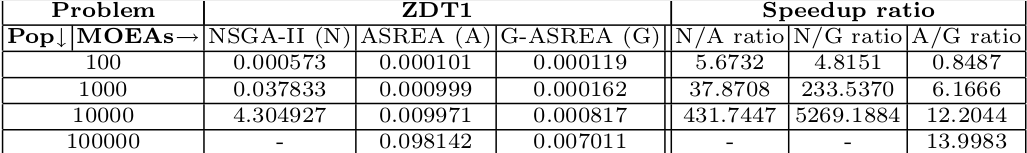
\includegraphics[width=6in]{img/asrea_table.png}
		\caption{Comparaison des temps et accélérations entre ASREA, NSGA-II et G-ASREA sur une minimisation de fonction ZDT\cite{zitzler2000comparison}.}
	\end{center}
\end{figure}
M. Collet m'a fourni une implémentation pour \textit{GPU} d'\emph{ASREA}. Le
code de l'algorithme était fortement imbriqué dans un programme de
benchmarking synthétique de \emph{GA} (\emph{ZDT functions\cite{zitzler2000comparison}}).

Nous avons continuer le travail de parallélisation sur \textit{G-ASREA} pour
qu'il soit exécuter en sont intégralité sur \textit{GPU}. Après extraction,
refactoring et adaptation, nous avons pu bénéficier d'accélérations
répertoriées dans la table suivante :

\begin{center}
	\begin{tabular}{ |l| c| r| }
		\hline
		Nombre d'individu & NSGA-II & G-ASREA \\
		\hline
		1024 & 5 ms & 2 ms \\
		16 384 & 464 ms & 19 ms\\
		32 768  & 1563 ms& 27 ms\\
		\hline
	\end{tabular}
	\captionof{table}{Temps de la sélection, moyennes sur 50 générations.}
\end{center}

\subsubsection{Execution time}
The main selling point of ASREA is its relatively low complexityO(man), one degree below that a NSGA O(n2). 
This permit much higher size of population resulting in a increase of diverstity. By having a high diversity 
among individual, the optimization is much better at avoiding local optimum and lessen the risk of premature 
convergence. NSGA-II is a purely sequencial algorithm and with high population count, represent as much as 
99,9\% of the execution time. Here is the speed-up of our implementation of ASREA over NSGA-II. \\
The results pretty much speak for themselves, we were able of getting almost 200 times faster generation 
than NSGA-II. Exhaustive benchmarking are provided in the table below.
 
\subsubsection{Quality of results}
An interesting byproduct of ASREA selection is the much better solution at a given generation while converging
in a much later stage of the evolution. This is due to the high diversity and the resilience to random mutation 
guarenteed by ASREA. Unfortunatly we had no time for a deeper analysis of this behaviours. Here are the plot of 
each fitness of the best solution at every generation of a run using ASREA against one using NSGA-II 

\subsection{Comparaison against human operators}
The direct comparaison of planning done by human operators against the one generated by the algorithm is difficult 
to survey directly. While human operators have difficulties visualizing the planning global order, that is the routing
 itself, they are also the one knowing about theirs company specificity and all the edge case not covered directly by 
the algorithm, i.e a patient only travel with a specific crew because of implicit reason (language, habit) or the company 
not allowing or favorising certain type of configuration.\\
\\
Thus the algorithm only serve as base plannification, that need to be review by an human operator in order to correct 
the obvious changes of specification. However, it does all the heavy lifting in a reasonable time (less than 1 minutes 
for the whole day) with the correction taking 5 to 10 minutes of midly intensive work, given that by hand, the same planning
should have took one hours of intensive work. When doing plannification with the help of the algorithm, one can expect a smaller 
cognitive workload and saving up to 3//4 of the needed time.  

\section{Deployement and architecture}

The current version of the deployed algorithm is the cpu version. This version is in
production in a few test clients, each one having very different needs. For example,
one client do not required to do any employee optimisation and its workload are
around the high-end of what we consider small client (~200), while the other need a
very precise and tight optimisation of theirs employee on small workload (~80).\\
\\
To be able to rapidly implement different features and toggles them on depending of the client,
we develop a small middleware in python django to launch instance of the algorithm
with the correct set of options. The middleware also take care of isolating the
different instances between users of the small company and serve as an orchestration
tools.\\
\\
The pipeline remains simple: the end-user configure than start the algorithm through
Saphir, Saphir than collect and export the data to the middleware. The middleware
then start the algorithm instances with the received data and addition options to
provide isolation.\\
\\
The GPGPU version while being done developed and tested, is still at the time of
writing not deployed due to the difficulty to get hardware equipped with specific
GPGPU in datacenter. We wanted to avoid having to pay for a dedicated server rack
with "professional-grade" GPGPU such as Tesla K20, because our algorithm was
designed with consumer-grade graphical card such as the Nvidia 960 GTX. Using the
cloud (Amazon AWS EC2) for this project is impossible due to the high tarification
of such services.
\\
We start using Docker for easy deployement and scalability of the algorithm. Docker
is a tool for deployement, orchestration and automatisation, providing a layer of
abstraction and isolation over the kernel and the linux operation system, in order
to avoid the problem related with virtual machine (slow starting time, size, etc
...). \\
Using Docker was quite informative about real-world deployement, robustness,
realtime scalability and monitoring. It is a tool that got a lot of praise those
last few year, but remains easy to use. Docker container are light (less than 500
MB for our), quick to deploy (a few minutes) and provide quasi-instantaneous launch
(around 300ms).

I still worked on deploying the architecture on Amazon Elastic Cloud as a back-up
solution. One of the only difficulty encounter is to get base amazo linux image with the
correct nvidia driver installed because it must correspond. To get a Docker
container correctly accessing the GPU, the toolkit install on it must also
correspond with the drivers installed on the host.
The price tag of Amazon EC2 is what block us from using it: The optimization must
run at all time in realtime continuous mode, and the average price of GPU instance
is around 0.3 dollars per hours, per client. 

\section{Role}

This year me role inside the company and in the project changed quite a bit. I kept
my position as the lead researcher and lead developer on the project, but I step
down for me position of junior project manager, for the following reason: due to the
algorithm going in product a lot control over the different tests and discution with
clients, modification or implementatin of feature were delegated to the main
hierarchy of the company. For a concrete example all communication with clients now
go through the support department, before going to the main project manager of
Saphir M. Munsch and occasionaly to the CTO M. Philips.\\
As the project did came to completion, more and more employee and fellower
developers of Synovo became familiar with the project, its goals, underlying
concepts and core functionalities.

\section{Discussion}

\section{Conclusion}

\bibliographystyle{plain}
\bibliography{thesis}

\end{document}
